\documentclass[letter,10pt]{article}
\usepackage[utf8]{inputenc}
\usepackage{graphicx}
\usepackage{natbib}
\usepackage{hyperref}
\usepackage{courier}
\usepackage[margin=0.75in]{geometry}
\usepackage[table,svgnames]{xcolor}
\usepackage{multirow}
\usepackage{tabu}
\usepackage{float}
\usepackage{listings}
\bibliographystyle{unsrtnat}
\definecolor{HeaderColor}{rgb}{0.8, 0.8, 0.95}
\setlength{\parindent}{0pt}
\setlength{\parskip}{6pt}

\graphicspath{{./figures/}}

\lstset{
    backgroundcolor=\color{white},
    tabsize=4,
    basicstyle=\ttfamily,
    breaklines=true
    framextopmargin=50pt,
    aboveskip={0.5\baselineskip},
    columns=fixed,
    frame=single,
    showstringspaces=false,
    extendedchars=false,
    breaklines=true,
    numbers=none,
    showtabs=false,
    showspaces=false,
    showstringspaces=false,
    identifierstyle=\color[rgb]{0.0,0.2,0.0},
    keywordstyle=\bfseries\color[rgb]{0.2,0.2,0.6},
    commentstyle=\color[rgb]{0.4,0.6,0.6},
    stringstyle=\color[rgb]{0.6,0.0,0.2},
    numberstyle=\tiny\color[rgb]{0.6, 0.6, 0.6}}

\lstdefinelanguage{dj}{
  keywords={int, smallint, char, varchar, enum, unsigned, date, year, decimal},
  keywordstyle=\color{blue},
  keywords=[2]{boolean, string, number, objectid},
  keywordstyle=[2]\color{green}\bfseries,
  identifierstyle=\color{black},
  sensitive=true,
  morecomment=[l][\color{teal}\bfseries]{::},
  morecomment=[l][\color{gray}\itshape\small]{\#},
  stringstyle=\color{red},
  morestring=[b]',
  morestring=[b]"
}

\newfloat{lstfloat}{htbp}{lop}
\floatname{lstfloat}{Listing}

\title{Re0: A Relational Data Language with Operational Entity Integrity.}
\author{Dimitri Yatsenko, Edgar Y.\ Walker}

\begin{document}

\maketitle
\begin{abstract}
A simplified and conceptually refined relational data model is proposed with a language for schema definition and data queries as well as a diagramming method for visualizing relationships among the data.  
Named Re0, the model adheres to the principle of \emph{operational entity integrity}, which requires that all data --- both stored and derived --- exist in the form of sets of entities belonging to well-defined entity classes.  
Re0's data query language is an algebra of five operators that provide equal capabilities to those of other relational query languages with greater clarity due to adherence to operational entity integrity. 
Practical implementations of Re0 known as DataJoint haves been tested and adopted for scientific data pipelines.  
With Re0, programmers interact with scientific data more fluently than with other data definition and query languages.
\end{abstract}
\tableofcontents 

\twocolumn

\section{The relational data model}
To motivate the need and the advantages of the proposed data model and query language, this section reviews the foundations and principles of the broader relational data model and the shortcomings of its present variants and implementations. 

\subsection{Foundations}
The relational data model \citep{codd_relational_1970} provides the most rigorous approach to structuring stored data and the most precise approach to querying stored data.  
Briefly, the relational data model is defined by the following principles:
\begin{enumerate}
\item Data are represented and manipulated in the form of \emph{relations}. 
A relation is a set of \emph{tuples} of values for the respective \emph{attributes} of the relation.
Relations may directly represent stored data \emph{(base relations)} or may be derived from stored data \emph{(derived relations)}.
\item Attribute values are drawn from corresponding attribute \emph{domains}, \emph{i.e.}\ predefined sets of values.
Attribute domains may not include other relations, ensuring that the relational model is essentially flat with no nesting data structures.
\item Tuples within relations are addressed by values of their attributes.
To identify and relate data elements, \emph{uniqueness constraints} on a subset of attributes may be imposed so that no two tuples can have the same values of these attributes.  The set of attributes with a uniqueness constraints are referred to as a \emph{key}. One in a relation key may be designated as the \emph{primary key} for the relation to serve for referencing elements in a relation.
\item Associations among data are established by means of \emph{referential constraints} in the form of \emph{foreign keys}. 
Referential constraints prohibit tuples in one relation that lack tuples with matching values in the referenced relation. 
\item \emph{Query expressions} produce derived relations from base relations.  Query expressions declare specifications for retrieving data.
Formal languages for query expressions include \emph{relational algebra} and \emph{relational calculus}.  
\end{enumerate}

A collection of base relations with their attributes, domains, uniqueness constraints, and referential constraints is commonly referred to as a database \emph{schema}.

The relational model itself is abstract and semantically unconstrained, allowing many distinct approaches for translating real-world entities and relationships into a relational database schema. 
A set of formal rules known as \emph{normal forms} have been defined to test whether a given schema meets basics quality requirements that minimize redundancies and anomalies in data manipulations \citep{kent-1983-simple}.
The relational model does not impose semantic constraints on its query expressions, giving freedom to equate arbitrary regardless of their semantics.

Different variants of the relational data model use different terminology to refer to similar concepts (Table \ref{tab:terms}).
\tabulinesep=6pt
\begin{table*}[ht]
   \rowcolors{1}{white}{gray!20}
   \begin{tabu}{|X[1,c,p]| X[1,c]| X[1,c]| X[1,c]|}
   \hline
   \rowcolor{HeaderColor}
   {\bf Relational} & {\bf ERM} & {\bf SQL} & {\bf Re0}  \\
   \cellcolor{white} & entity set & \cellcolor{white} & \cellcolor{white} \\
   \multirow{-2}{*}{relation}  & relationship set  & \multirow{-2}{*}{table}  &  \multirow{-2}{*}{entity set} \\
   tuple       & entity           & row       & entity \\
   domain      & value set        & data type & data type \\
   attribute   & attribute        & column {\em or} field    & attribute \\
   attribute value & attribute value  & field value & attribute value \\
   primary key & primary key & primary key & primary key \\
   foreign key & foreign key & foreign key & foreign key \\
   relational expression \par {\em or} derived relation &  data query & {\tt SELECT} statement & query expression \\
   \hline
   \end{tabu}
\caption{Corresponding terms used in variants of relational models.}
\label{tab:terms}
\end{table*}

\subsection{SQL}
Common implementations of the relational data model rely on the Structured Query Language (SQL) for schema definition and data queries.
SQL so thoroughly dominates in the space of relational databases that it has become nearly synonymous with the relational data model despite its deviations from it. 
Effectively, SQL implements a distinct variant of the relational data model that allows its use in non-relational ways. 
Since SQL is the effective lingua franca in the world of relational databases, some examples and discussions will explicitly highlight the principal conceptual weaknesses of SQL that are resolved with Re0.

\subsection{ERM}
Peter Chen \citep{chen_entity_1976} proposed the Entity-Relationship Model (ERM) to conceptually clarify the relational data model.
In the ERM, each base relation denotes either a set of entities or a set of relationships between sets of entities. 
Each entity set may contain entities of the same class, sharing the same set of attributes and distinguished by the same  primary key.
Foreign keys between relationship sets and entity sets express and enforce the corresponding relationship.

In ERM, query expressions follow patterns established through relationship sets between entity sets, providing a correspondence between the schema design and sensible queries. 
The development of ERM stopped short of defining a formal query language distinct from those of the broader relational model.

Despite its origin as a relational data model in its own right, ERM is now taught as an abstract model for \emph{conceptual modeling} with expressive diagramming notation.  
Modern introductory texts and courses on relational databases distinguish \emph{conceptual modeling} from \emph{logical design} as separate phases of database design and implementation \citep{elmasri-2015-fundamentals, coronel-2016-database}.
SQL does not explicitly embody ERM, practicing programmers internalize its concepts and  mentally or explicitly categorize tables as either ``entity tables'' or ``relationship tables''.  
ERM designs tend to produce database schemas that already  meet rules of database normalization from formal relational database theory and practicing database developers rarely need to recall the definitions of normal forms from their formal academic training.

\subsection{Entity integrity}
In the ERM, an entity is defined as distinct and identifiable within its entity set. 

The \emph{entity integrity} constraint is the requirement that relations must have an explicit primary key and that values of the primary key attributes cannot be null. 

\section{Re0 Foundations}
Re0 provides a simpler, conceptually refined relational data model that is as expressive as it is practical. 
It eliminates the gap between conceptual modeling and logical design in database development.

Re0 consists of a schema definition language, a data query language, and diagramming notation for visualizing relationships between data elements. 

The central concept of the Re0 data model is that of an \emph{entity set}. 
An entity set is an unordered collection of distinct \emph{entities} of the same \emph{entity class}.
An individual entity is an object, an item, or a more abstract entity (\emph{e.g.}\ a relationship) that is distinctly identified in the model universe. 
All entities in the same entity class have the same attributes and the same primary key.

This definition entity set is essentially identical to that of the Entity-Relationship Model.

\section{Schema Definition --- Basics.}\label{sec:basic}
In this section, we will describe the \emph{schema definition language} of Re0.

\subsection{Entity-set declaration}
A schema is defined by declaring a collection of \emph{base entity sets}.
An entity set is a set of distinct and identifiable entities from the model world. 
A base entity has a unique name within the schema 

\begin{lstfloat*}
\begin{lstlisting}[language=dj]
::Student     
student_id : int unsigned   # university-wide ID number 
---
first_name      : varchar(40)
last_name       : varchar(40)
sex             : enum('F', 'M', 'U')
date_of_birth   : date
student_address : varchar(200) # mailing address
student_phone   : varchar(14) 

::Department 
dept : varchar(6)   # abbreviated department name, e.g. BIOL
---
dept_name    : varchar(200)  # full department name
dept_address : varchar(200)  # mailing address
dept_phone   : varchar(14)  

::StudentMajor
-> Student
---
-> Department
declare_date :  date  # when student declared her major  
\end{lstlisting}
\caption{University database schema definition (Part 1).}
\end{lstfloat*}

\begin{lstfloat*}
\begin{lstlisting}[language=dj]
::Course     
-> Department
course  : int unsigned   # course number, e.g. 1010
---
course_name :  varchar(200)  # e.g. "Neurobiology of Sensation and Movement."
credits     :  decimal(3,1)  # number of credits earned by completing the course

::Term
term_year : year 
term      : enum('Spring', 'Summer', 'Fall')

::Section 
-> Course
-> Term 
section : char(1)
---
auditorium   :  varchar(12)

::CurrentTerm
---
-> Term

::Enroll
-> Section
-> Student 

::LetterGrade
grade : char
---
points : decimal(3,2)

::Grade 
-> Enroll
---
-> LetterGrade

\end{lstlisting}
\caption{University database schema definition (Part 2).}
\end{lstfloat*}

\begin{figure}
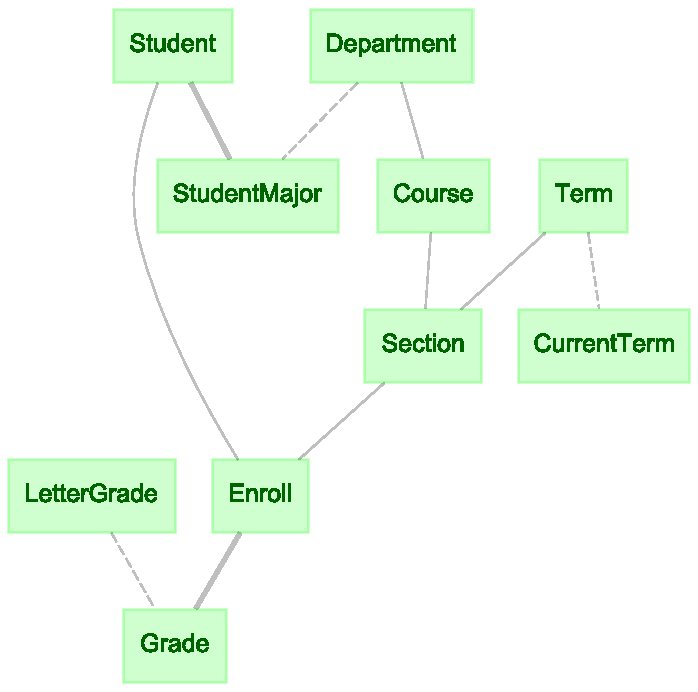
\includegraphics[width=\columnwidth]{uni_erd.pdf}
\caption{The schema diagram of the university database.}
\label{fig:erd}
\end{figure}


\subsubsection{Attributes and their datatypes}
\subsubsection{Primary key}

\subsection{Dependencies}
\subsubsection{Effects of dependencies}
\subsubsection{Primary and secondary dependencies}
\subsubsection{Acyclicity}

\subsection{Schema diagrams}

\section{Data manipulation}
\subsection{Insert}
\subsection{Delete}
\subsection{Cautious update}

\section{Query Expressions}
\subsection{Relational operators and expressions}
\subsection{Operational entity integrity}
\subsection{Join compatibility}
\subsection{Restriction}
\subsubsection{Restriction by attribute conditions}
\subsubsection{Restriction by other relations}
\subsubsection{Restriction by a list}

\subsection{Join}
\subsection{Projection}
\subsection{Union}
\subsection{Aggregation}
Aggregation functions cannot be used in restrictions. 
\subsection{Relation U}

\section{Schema Definition --- Advanced.}
\subsection{Dependencies on query expressions}
\subsection{Master-part relationship}
The primary motivation for the master-part relationship is to inform the application that the master and all its parts should always appear together or not at all.  
This usually means using transactions.  
A transaction starts then the master is inserted, then all the parts, and only then the transaction is committed.  
This way all other users only see the master entry when all its parts have been entered.
A part may be in 1-to-1 relationship with its master without any new primary attributes.
\subsection{Dependency properties}

\appendix

\section{Differences from SQL}
Faithful adherence to the relational data model. 
Native entity integrity.

\subsection{SQL Translations}


\bibliography{DataJoint}

\end{document}
